% This must be in the first 5 lines to tell arXiv to use pdfLaTeX, which is strongly recommended.
\pdfoutput=1
% In particular, the hyperref package requires pdfLaTeX in order to break URLs across lines.

\documentclass[11pt]{article}

% Remove the "review" option to generate the final version.
\usepackage[review]{EMNLP2022}

% Standard package includes
\usepackage{times}
\usepackage{latexsym}

% For proper rendering and hyphenation of words containing Latin characters (including in bib files)
\usepackage[T1]{fontenc}
% For Vietnamese characters
% \usepackage[T5]{fontenc}
% See https://www.latex-project.org/help/documentation/encguide.pdf for other character sets

% This assumes your files are encoded as UTF8
\usepackage[utf8]{inputenc}

% This is not strictly necessary, and may be commented out.
% However, it will improve the layout of the manuscript,
% and will typically save some space.
\usepackage{microtype}

% This is also not strictly necessary, and may be commented out.
% However, it will improve the aesthetics of text in
% the typewriter font.
\usepackage{inconsolata}

\usepackage{graphicx}
\usepackage{amsfonts}
\usepackage{amsmath}
\usepackage{amssymb}
\usepackage{bbm}
\usepackage{backnaur}

\renewcommand{\bnfpn}[1]{\mathsf{#1}}
\renewcommand{\bnfpo}{\rightarrow}
\renewcommand{\bnfts}[1]{\mathtt{#1}}



% If the title and author information does not fit in the area allocated, uncomment the following
%
%\setlength\titlebox{<dim>}
%
% and set <dim> to something 5cm or larger.

\title{Towards More Natural Artificial Languages}

% Author information can be set in various styles:
% For several authors from the same institution:
% \author{Author 1 \and ... \and Author n \\
%         Address line \\ ... \\ Address line}
% if the names do not fit well on one line use
%         Author 1 \\ {\bf Author 2} \\ ... \\ {\bf Author n} \\
% For authors from different institutions:
% \author{Author 1 \\ Address line \\  ... \\ Address line
%         \And  ... \And
%         Author n \\ Address line \\ ... \\ Address line}
% To start a seperate ``row'' of authors use \AND, as in
% \author{Author 1 \\ Address line \\  ... \\ Address line
%         \AND
%         Author 2 \\ Address line \\ ... \\ Address line \And
%         Author 3 \\ Address line \\ ... \\ Address line}

\author{First Author \\
  Affiliation / Address line 1 \\
  Affiliation / Address line 2 \\
  Affiliation / Address line 3 \\
  \texttt{email@domain} \\\And
  Second Author \\
  Affiliation / Address line 1 \\
  Affiliation / Address line 2 \\
  Affiliation / Address line 3 \\
  \texttt{email@domain} \\}

\begin{document}
\maketitle
\begin{abstract}
A number of papers have recently argued in favor of using artificially generated languages to investigate the inductive biases of linguistic models, or to develop models for low-resource languages with underrepresented typologies. But the promise of artificial languages comes with a caveat: if these artificial languages are not sufficiently reflective of natural language, then using them as a proxy may lead to inaccurate conclusions. In this paper, we take a step towards increasing the realism of artificial language by introducing a variant of indexed grammars that draw their weights from hierarchical Pitman-Yor processes. We show that this framework generates languages that emulate the statistics of natural language corpora better than the current approach of directly formulating weighted context-free grammars. 
\end{abstract}

\section{Introduction}

In the World Atlas of Linguistic Structures, \citet{wals81} reports that the plurality of world languages follow a subject-object-verb (SOV) word order. However, relatively few SOV languages (Japanese, Turkish, Persian) have a significant Internet footprint. Today, the Internet is dominated by subject-verb-object (SVO) languages like English, Spanish, and Chinese. The resulting paucity of non-SVO data makes it difficult to study whether linguistic models have an inductive bias towards particular word orders, or to develop models that perform well on low-resource languages from underrepresented linguistic families. In recent work, \citet{wang-eisner-2016-galactic}, \citet{ravfogel-etal-2019-studying} and \citet{white-cotterell-2021-examining} argue that artificial languages could be an effective tool for addressing challenges like these, enabling researchers to create large corpora that manifest targeted linguistic phenomena.

An obvious objection presents itself: what if the models aren't realistic enough? If not, then conclusions drawn from artificial languages may not transfer to natural languages. One response to this objection would be to abandon the entire enterprise, and with it the potential advantages of simulated data. An alternative is to follow the tradition of other disciplines who model natural systems (e.g. physics, geology, meteorology) and iterate on these models until they are sufficiently good predictors of observed phenomena.

In this spirit, this paper builds upon the framework of \citet{white-cotterell-2021-examining}, who used weighted context-free grammars to construct artificial languages for studying the inductive biases of neural language models towards particular word orders. Observing that their framework did not account for selectional preference (the linguistic  phenomenon that head words and their syntactic dependents are not probabilistically independent), we generalize weighted context-free grammars by introducing the \emph{weighted random-access indexed grammar}, which facilitates the development of artificial languages that manifest selectional preference.


\begin{figure*}[tb]
\centering
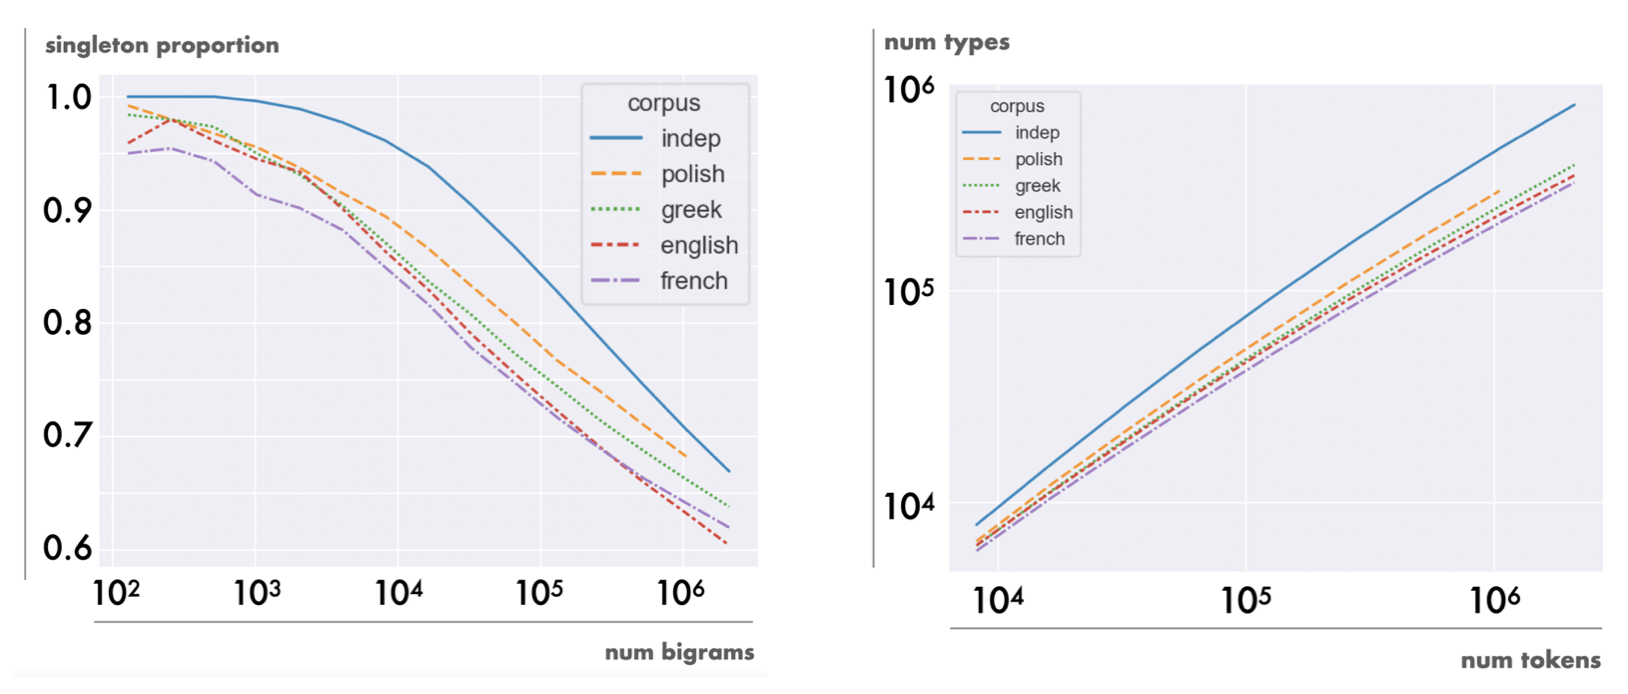
\includegraphics[width=0.92\textwidth]{images/demo_plots.png}
\caption{A comparison of the singleton proportion curves of adjective-noun bigrams in the Europarl corpus with bigrams generated using independent adjective and noun distributions.}
\label{fig:motivationcurve}
\end{figure*}


%\begin{figure}[tb]
%\begin{bnf*}
%\bnfprod{S} {\bnfpn{NN} \bnfsp \bnfpn{VP}} \\
%\bnfprod{VP} {\bnfpn{VB} \bnfsp \bnfpn{NN}}\\
%\bnfprod{VB} {\bnfts{drank} \bnfor \bnfts{ate}} \\
%\bnfprod{NN} {\bnfts{you} \bnfor \bnfts{it} \bnfor \bnfts{water} \bnfor \bnfts{food}}
%\end{bnf*}
%\caption{A CFG describing a small subset of English.\label{fig:pcfg1}}
%\end{figure}


We also present a methodology for building grammars that emulate statistical relationships observed in natural language corpora. Inspired by \citet{teh-2006-hierarchical}, we use hierarchical Pitman-Yor processes \cite{pitman1997two} as the token-generating distributions for open-class categories (like noun, verb, and adjective). We set the hyperparameters by matching the statistics of the produced artificial languages with natural language corpora.

As a pilot experiment for our framework, we replicate an experiment performed by \citet{white-cotterell-2021-examining} that studied the inductive bias of transformer and LSTM-based language models towards languages featuring various syntactic parameter configurations \cite{chomsky1981principles,baker2008atoms}.

Finally, we accompany this paper with an open-source Python package called \texttt{testperanto}, to allow researchers to use and refine our framework for further linguistic studies.

\section{Related Work}


Both \citet{wang-eisner-2016-galactic} and \citet{ravfogel-etal-2019-studying} constructed artificial languages by manipulating sentences from existing natural language corpora. Both approaches made use of a dependency parser (or a gold parsed corpus) to inform these manipulations, altering syntactic constituent order \cite{wang-eisner-2016-galactic,ravfogel-etal-2019-studying} or token morphology \cite{ravfogel-etal-2019-studying}. 

\citet{white-cotterell-2021-examining} argued that manipulated natural language corpora have downsides. Based on a series of negative results \cite{cotterell-etal-2018-languages,mielke-etal-2019-kind}, they suggested that it may not be possible to remove confounding linguistic features from an existing corpus, making it difficult to isolate typological features for study. To maximize the ability to run a controlled experiment, they generated fully artificial languages from hand-built weighted context-free grammars. However, although their grammars modeled certain syntactic dependencies (e.g. conjugating a verb with its subject), they did not model semantic dependencies. We assert that it is prohibitively difficult to directly formulate weighted context-free grammars that model semantic dependencies (e.g. selectional preference), motivating our extension -- the weighted random-access indexed grammar. 

%Other papers leveraging manipulated natural language to study model performance or linguistic phenomena include \citet{pmlr-v80-lake18a} and \citet{cogsci18-McCoy}. Other papers that have used generated languages (albeit with a narrow scope) to study model performance include \citet{DBLP:journals/corr/BowmanMP15} and \citet{DBLP:journals/corr/WestonBCM15}.




\section{Motivation}



\citet{white-cotterell-2021-examining} generated artificial language using a \emph{weighted context-free grammar} (WCFG). A WCFG augments a context-free grammar (CFG) with a function $q$ that assigns a nonnegative weight $q(r)$ to each grammar rule $r$. This induces a weight for each derivation: the product of the weights of the rules used in the derivation. More formal details can be found in \citet{collins2013lexicalized}. 

WCFGs produce terminal symbols (words) according to probability distributions that depend exclusively on the grammar nonterminals. Consider the following CFG:
\begin{bnf*}
\bnfprod{S} {\bnfpn{NN} \bnfsp \bnfpn{VP}} \\
\bnfprod{VP} {\bnfpn{VB} \bnfsp \bnfpn{NN}}\\
\bnfprod{VB} {\bnfts{drank} \bnfor \bnfts{ate}} \\
\bnfprod{NN} {\bnfts{you} \bnfor \bnfts{it} \bnfor \bnfts{water} \bnfor \bnfts{food}}
\end{bnf*}
By using plain nonterminals like $\bnfpn{VB}$ and $\bnfpn{NN}$, the respective probabilities of sentences $\bnfts{it} \bnfsp \bnfts{drank} \bnfsp \bnfts{water}$ and $\bnfts{it} \bnfsp \bnfts{drank} \bnfsp \bnfts{food}$ depend only on the probability of the rules $\bnfpn{VB} \bnfpo \bnfts{water}$ and $\bnfpn{VB} \bnfpo \bnfts{food}$. Crucially, the verb choice does not differentiate the sentence probabilities. This is unrealistic -- it is more common to drink water than to drink food, whereas it is more common to eat food than to eat water. This phenomenon (that linguistic arguments are not independent of their predicates) is known as \emph{selectional preference}.

\begin{figure}[t]
\centering
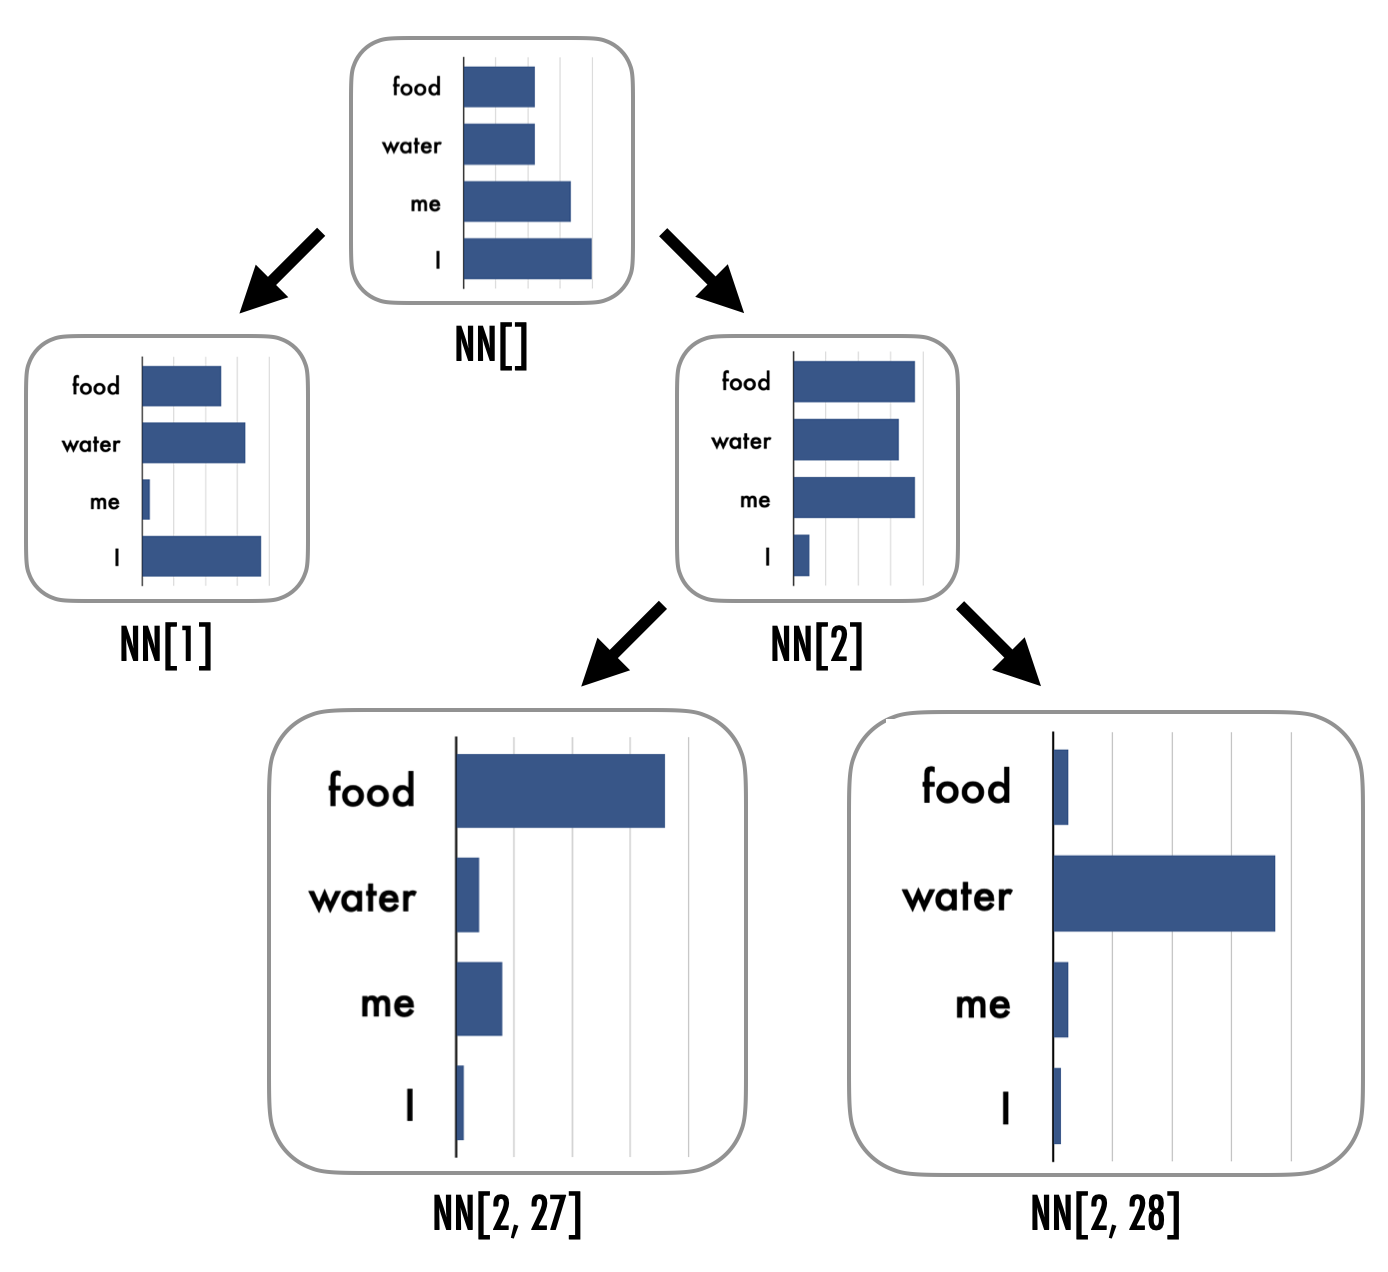
\includegraphics[width=0.48\textwidth]{images/hierarchical_process.png}
\caption{An example hierarchical Pitman-Yor process. $\bnfpn{NN[]}$ is the global noun distribution. $\bnfpn{NN[1]}$ and $\bnfpn{NN[2]}$ respectively represent the likelihood that a noun is the subject or object of a verb. $\bnfpn{NN[2, 27]}$ and $\bnfpn{NN[2, 28]}$ respectively represent the likelihood that a noun is the object of verb 27 (eat) or verb 28 (drink) of the vocab.}
\label{fig:hierarchical_process}
\end{figure}


One way to detect selectional preference \cite{teh-2006-hierarchical} is to collect dependency relationships from a parsed natural language corpus (e.g. \texttt{amod}, \texttt{nsubj}, \texttt{dodj}) and extract the dependency bigrams (e.g. for \texttt{amod}, the first three dependency bigrams in Europarl are \texttt{internal market}, \texttt{European citizens}, and \texttt{cultural exception}). Then, as we stream through the dependency bigrams, we plot either the number of observed bigram types (a type-token curve) or the proportion of bigrams whose type has been observed exactly once (a singleton proportion curve). In Figure~\ref{fig:motivationcurve}, we contrast the curves generated\footnote{To generate Figure~\ref{fig:motivationcurve}, we shuffled the Europarl sentences and extracted the adjective-noun dependencies using \texttt{spaCy}. The shuffling smooths irregularities caused by topic shift.} using four Europarl corpora \cite{koehn-2005-europarl} with a bigram corpus constructed by sampling one adjective and one noun from independent distributions respectively derived from adjective and noun frequency in the English Europarl corpus. The curves generated using the independent bigram corpus are outliers. For instance, when the number of observed bigrams is plotted on a log scale, the natural corpora have roughly linear singleton proportion curves, whereas the independent corpus has a considerable bow in the curve.

We would like to generate artificial languages such that the dependencies have similar statistics to naturally observed dependencies. Rather than independently generating open-class words, \citet{teh-2006-hierarchical} suggests using a hierarchical Pitman-Yor process \cite{pitman1997two} -- a tree-structured set of distributions over the same domain, in which child distributions are resamplings of their parents. Figure~\ref{fig:hierarchical_process} shows an example. A hierarchical Pitman-Yor process allows us to model context-specific word distributions (e.g. \texttt{food} is more likely to appear as the object of the verb \texttt{eat} than \texttt{water}, \texttt{I}, or \texttt{me}) that are jointly influenced by global word frequency priors. A Pitman-Yor process $\mathsf{PY}(d, \theta, P_{\mathsf{base}})$ is characterized by a \emph{discount} parameter $d \in [0,1)$, a \emph{strength} parameter $\theta \in (-d,\infty)$, and a \emph{base distribution} $P_{\mathsf{base}}$ over integers $\{1, \dots, V\}$. We follow \cite{teh-2006-hierarchical} in describing a Pitman-Yor process as a stochastic process that generates samples $\langle x_1, x_2, ... \rangle$ from i.i.d. samples $\langle y_1, y_2, ... \rangle$ drawn from base distribution $P_{\mathsf{base}}$. Intuitively, it is a ``rich-get-richer'' process, in which the $j$th sample $x_j$ is set to either the value $y_i$ assigned to a previous $x$-sample (with probability proportional to the number of previous $x$-samples that were assigned the value $y_i$), or the next $y$-sample in the sequence that hasn't yet been used. Formally, let $b_1=1$ and draw subsequent binary values $b_{n+1}$ from a Bernoulli (coin-flip) distribution where:
\begin{equation*}
	P(b_{n+1} = 1) =\frac{\theta + d\sum\limits_{1 \leq i \leq n} b_i}{\theta + n} 
\end{equation*}

\noindent Variable $b_{n+1}$ determines whether the $(n+1)$th sample is set to the value of a previous assignment ($b_{n+1}=0$) or the next unused $y_i$ sample ($b_{n+1}=1$). Now define $t_1 = 1$ and consider $j, n \in \mathbb{Z}^+$. If $b_{n+1}=0$, then let $t_{n+1}=j$ with probability:
\begin{equation*}
	\frac{1}{n} \sum\limits_{1 \leq i \leq n} \mathbbm{1}(t_i=j)
\end{equation*}
Otherwise, if $b_{n+1}=1$: 
\begin{equation*}
t_{n+1}=1 + \sum\limits_{1 \leq i \leq n} b_i
\end{equation*}

\noindent The $n$th sample drawn from the Pitman-Yor process is $x_n = y_{t_n}$. A Pitman-Yor process, for all practical purposes, can generate an ``open-class'' of words by using a uniform base distribution $P_{\mathsf{unif}}$ with a sufficiently large vocabulary size $V$ (for our experiments, we use the space of all 32-bit integers). 

A hierarchical Pitman-Yor process is simply a Pitman-Yor process that uses another Pitman-Yor process as its base distribution. For instance, we could define a global adjective distribution $P_\mathsf{adj} = \mathsf{PY}(0.4, 500, P_{\mathsf{unif}})$, and then for noun $\bnfpn{y_1}$ of our vocabulary, we could define a noun-dependent adjective distribution $P_\mathsf{\bnfpn{adj, y_1}} = \mathsf{PY}(d, \theta, P_\mathsf{adj})$. 





\section{Approach}

The main challenge: how do we construct a WCFG that derives its weights from the linked distributions of a hierarchical Pitman-Yor process? Concerned with the induction of better n-gram language models, previous work \cite{teh-2006-hierarchical,blunsom-cohn-2011-hierarchical} mainly focused on how to incorporate hierarchical Pitman-Yor processes into sequential models like Hidden Markov Models. Here, our concern is how to incorporate these distributions into a generative syntactic model convenient for engineering artificial languages with specific linguistic typologies. There exist many syntactic models to choose from, including dependency grammars \cite{eisner-1996-three}, tree-adjoining grammars \cite{joshi1987introduction}, lexical functional grammars \cite{kaplan-1985-structural}, CCGs \cite{steedman2011combinatory}, HPSGs \cite{pollard1994head} and GPSGs \cite{gazdar1985generalized}. In this work, we choose to extend context-free grammars, partly because of their popularity and partly to facilitate comparison with \cite{white-cotterell-2021-examining}, who used WCFGs -- however, our approach can be adapted to other syntactic formalisms.


%One approach is to refine the nonterminals with indices that encode the choice of syntactic head \cite{collins-1997-three} or head class \cite{klein-manning-2003-accurate}. Given an appropriate refinement (for instance, Figure~\ref{fig:pcfg3}), we can now assign a high probability to the rule $\bnfpn{VP.28} \bnfpo \bnfpn{VB.28} \bnfsp \bnfpn{NN.57}$ (because it common to drink water) and a low probability to the rule $\bnfpn{VP.28} \bnfpo \bnfpn{VB.28} \bnfsp \bnfpn{NN.56}$ (because it is uncommon to drink food). Unfortunately, the prospect of directly engineering such a grammar is daunting. Previous work on grammars with refined nonterminals \cite{collins-1997-three,klein-manning-2003-accurate,matsuzaki-etal-2005-probabilistic} focused largely on how to automatically induce refined grammars from natural language corpora, not on how to generate artificial language with realistic statistics. In the next section, we propose a lightweight extension of a WCFG specifically for the generation of ``natural'' artificial language.





%\begin{figure}[t]
%\begin{bnf*}
%\bnfprod{S} {\bnfpn{S[27]} \bnfor \bnfpn{S[28]}} \\
%\bnfprod{S[27]} {\bnfpn{NN[9]} \bnfsp \bnfpn{VP[27]}} \\
%\bnfprod{S[28]} {\bnfpn{NN[9]} \bnfsp \bnfpn{VP[28]}} \\
%\bnfprod{VP[27]} {\bnfpn{VB[27]} \bnfsp \bnfpn{NN[56]}}\\
%\bnfprod{VP[27]} {\bnfpn{VB[27]} \bnfsp \bnfpn{NN[57]}}\\
%\bnfprod{VP[28]} {\bnfpn{VB[28]} \bnfsp \bnfpn{NN[56]}}\\
%\bnfprod{VP[28]} {\bnfpn{VB[28]} \bnfsp \bnfpn{NN[57]}}\\
%\bnfprod{VB[27]} {\bnfts{ate}} \\
%\bnfprod{VB[28]} {\bnfts{drank}} \\
%\bnfprod{NN[9]} {\bnfts{it}}\\
%\bnfprod{NN[56]} {\bnfts{food}}\\
%\bnfprod{NN[57]} {\bnfts{water}}
%\end{bnf*}
%\caption{A refinement of the CFG from Figure~\ref{fig:pcfg1} to model selectional preference.\label{fig:pcfg3}}
%\end{figure}



\begin{figure}[t]
\centering
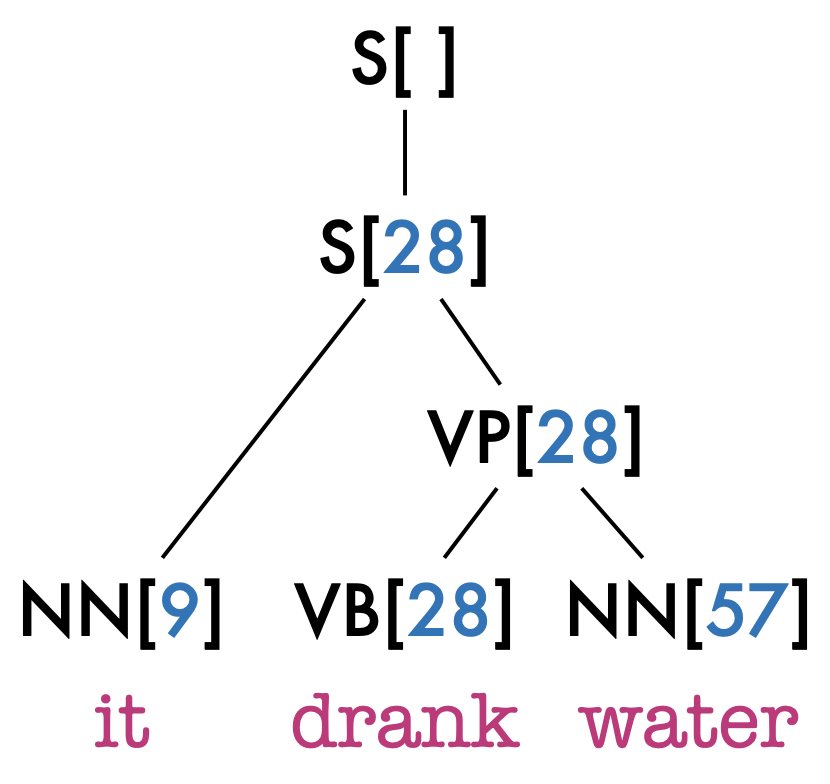
\includegraphics[width=0.36\textwidth]{images/derivation2.png}
\caption{An example derivation, using the indexed grammar from Figure~\ref{fig:indexed_grammar}.}
\label{fig:derivation}
\end{figure}

%\begin{figure}[t]
%\begin{bnf*}
%\bnfprod{S[]} {\bnfpn{S[z_1]}} \\
%\bnfprod{S[y_1]} {\bnfpn{NN[z_1]} \bnfsp \bnfpn{VP[y_1]}} \\
%\bnfprod{VP[y_1]} {\bnfpn{VB[y_1]} \bnfsp \bnfpn{NN[z_1]}}\\
%\bnfprod{VB[27]} {\bnfts{ate}} \\
%\bnfprod{VB[28]} {\bnfts{drank}} \\
%\bnfprod{NN[9]} {\bnfts{it}}\\
%\bnfprod{NN[56]} {\bnfts{food}}\\
%\bnfprod{NN[57]} {\bnfts{water}}
%\end{bnf*}
%\caption{An example indexed grammar.\label{fig:indexed_grammar}}
%\end{figure}

\begin{figure}
\begin{tabular}{rcl|l} 
&&&$\zeta$\\
\hline \hline
$\bnfpn{S[]}$ &$\bnfpo$& $\bnfpn{S[z_1]}$ & $\bnfpn{z_1} \mapsto \bnfpn{VB[]}$ \\
$\bnfpn{S[y_1]}$ &$\bnfpo$& $\bnfpn{NN[z_1]} \bnfsp \bnfpn{VP[y_1]}$ &  $\bnfpn{z_1} \mapsto \bnfpn{NN[1, y_1]}$\\
$\bnfpn{VP[y_1]}$ &$\bnfpo$& $\bnfpn{VB[y_1]} \bnfsp \bnfpn{NN[z_1]}$ &  $\bnfpn{z_1} \mapsto \bnfpn{NN[2, y_1]}$\\
$\bnfpn{VB[27]}$ &$\bnfpo$& $\bnfts{ate}$ & \\
$\bnfpn{VB[28]}$ &$\bnfpo$& $\bnfts{drank}$ & \\
$\bnfpn{NN[9]}$ &$\bnfpo$& $\bnfts{it}$ & \\
$\bnfpn{NN[56]}$ &$\bnfpo$& $\bnfts{food}$ & \\
$\bnfpn{NN[57]}$ &$\bnfpo$& $\bnfts{water}$ & 
\end{tabular}
\caption{An example indexed grammar. The base weight $w_0(\rho)$ of each indexed rule $\rho$ is 1.\label{fig:indexed_grammar}}
\end{figure}


\subsection{Intuition}

Our approach is a variation on indexed grammars \cite{aho1968indexed,hopcroft2001introduction}, which augment CFG nonterminals with a sequence of symbols called \emph{indices}. Before going through the formalism, we briefly preview how it works, using a derivation (Figure~\ref{fig:derivation}) for an example indexed grammar (Figure~\ref{fig:indexed_grammar}). At the top level, it applies CFG rule $\bnfpn{S[]} \bnfpo \bnfpn{S[28]}$, which involves two choices: 
\begin{enumerate}
	\item the choice of ``indexed rule": $\bnfpn{S[]} \bnfpo \bnfpn{S[z_1]}$
	\item the choice of indices to assign to its $z$-variables:  $\{ \bnfpn{z_1} \mapsto 28 \}$
\end{enumerate}
Next, the derivation expands $\bnfpn{S[28]}$ by applying the CFG rule $\bnfpn{S[28]} \bnfpo \bnfpn{NN[9]} \bnfsp \bnfpn{VP[28]}$. Again, this involves two choices: 
\begin{enumerate}
	\item the choice of indexed rule: $\bnfpn{S[y_1]} \bnfpo \bnfpn{NN[z_1]} \bnfsp \bnfpn{VP[y_1]}$
	\item the choice of indices to assign to its $z$-variables: $\{ \bnfpn{z_1} \mapsto 9 \}$
\end{enumerate}
Note the role of the variables: $\bnfpn{y}$-variables match LHS indices and copy them to the RHS, whereas $\bnfpn{z}$-variables introduce new indices on the RHS. Each $\bnfpn{z}$-variable $\bnfpn{z_i}$ of an indexed rule is associated with a key $\zeta(z_i)$ (Figure~\ref{fig:indexed_grammar}, right column) that references a distribution in a ``distribution table'' $\tau$. The weight associated with a derivation rule (e.g. $\bnfpn{S[28]} \bnfpo \bnfpn{NN[9]} \bnfsp \bnfpn{VP[28]}$) is the product of the base weight $w_0$ of the indexed rule (e.g. $w_0(\bnfpn{S[y_1]} \bnfpo \bnfpn{NN[z_1]} \bnfsp \bnfpn{VP[y_1]})$, and the probabilities of the $\bnfpn{z}$-assignments (e.g. $\tau(\mathsf{NN[1,28]})(9)$). As with CFGs, the weight of a derivation is the product of the derivation rules.




\subsection{Random-access Indexed Grammars}

Let $Y = \{\bnfpn{y_1}, \bnfpn{y_2}, ...\}$ and $Z = \{\bnfpn{z_1}, \bnfpn{z_2}, ...\}$ be reserved symbols called $\bnfpn{y}$- and $\bnfpn{z}$-variables. A \emph{random-access indexed grammar (RIG)}\footnote{The standard definition of indexed grammars \cite{hopcroft2001introduction} treats the indices as a stack, rather than as a random-access array. Our departure from the standard definition (introducing $\bnfpn{y}$- and $\bnfpn{z}$-variables to allow random-access matching) prioritizes the ease of grammar engineering over definitional conciseness and representational power. Moreover, since our use case is generation, we are not concerned with indexed grammar variants that prioritize efficiency of parsing or induction (e.g. \cite{gazdar-1987-comit}).} is a 5-tuple $(N, T, F, S, R)$ where:
\begin{itemize}
	\item $N$ is a set of \emph{nonterminal} symbols
	\item $T$ is a set of \emph{terminal} symbols
	\item $F$ is a set of \emph{index} symbols, or \emph{indices}\footnote{In this paper, we will use the set of nonnegative 32-bit integers as our set $F$ of indices.}
	\item $S \in N$ is the \emph{start symbol}
	\item $R$ is a finite set of \emph{indexed rules} (to be defined shortly)
\end{itemize}
In contrast to standard CFG rules, indexed rules use \emph{indexed nonterminals}, symbols of the form $\bnfpn{A[\phi]}$, where $\bnfpn{A} \in N$ and $\bnfpn{\phi} \in (F \cup Y \cup Z)^*$. A \emph{grounded indexed nonterminal} is an indexed nonterminal $\bnfpn{A[\phi]}$ such that $\bnfpn{\phi} \in F^*$. An \emph{indexed rule} has the form:
\begin{equation*}
	\bnfpn{A[\phi]} \bnfpo \bnfpn{rhs}
\end{equation*}
where $\bnfpn{A[\phi]}$ is an indexed nonterminal without $\bnfpn{z}$-variables, and $\bnfpn{rhs}$ is a sequence of terminals and indexed nonterminals whose $\bnfpn{y}$-variables all appear in $\phi$.

To define the semantics of a RIG, let a \emph{substitution} be a function $\sigma: D \rightarrow F$ with domain $D \subseteq Y \cup Z$. We apply a substitution $\sigma$ to a indexed nonterminal $\bnfpn{A[\phi_1, \dots, \phi_n]}$ as follows:
\begin{equation*}
\sigma(\bnfpn{A[\phi_1, \dots, \phi_n]}) = \bnfpn{A[\bar{\sigma}(\phi_1), \cdots, \bar{\sigma}(\phi_n)]}
\end{equation*}
where:
\begin{gather*}
\bar{\sigma}(x) = \begin{cases}
         \sigma(x) &\mbox{ if } x \in D\\
         x &\mbox{ if } x \not\in D
       \end{cases}
\end{gather*}
\noindent for $x \in F \cup Y \cup Z$. We apply a substitution $\sigma$ to an indexed rule $\rho$ by applying $\sigma$ to every indexed nonterminal in $\rho$.
For example, if:
\begin{eqnarray*}
	\sigma &=& \{ \bnfpn{y_1} \mapsto 52, \bnfpn{z_1} \mapsto 14 \} \\
	\rho &=& \bnfpn{S[y_1]} \bnfpo \bnfpn{NN[z_1]} \bnfsp \bnfpn{VP[y_1]}
\end{eqnarray*} 
then:
\begin{equation*}
\sigma(\rho) = \bnfpn{S[52]} \bnfpo \bnfpn{NN[14]} \bnfsp \bnfpn{VP[52]}
\end{equation*}



\noindent Each indexed rule $\rho$ implicitly represents the set of CFG rules that can be obtained by applying a substitution to the variables of the indexed rule:
\begin{equation*}
	\mathcal{R}(\rho) = \{\sigma(\rho) \mid \sigma: V(\rho) \rightarrow F \}
\end{equation*}
Here, $V(\rho) \subseteq Y \cup Z$ is the set of variables that appear in indexed rule $\rho$. The RIG encodes a CFG consisting of the union $\bigcup_{\rho \in R} \mathcal{R}(\rho)$ of these rules.

%The second difference is that the terminal rules generate generic words like $\bnfts{verb.3.1}$ and $\bnfts{verb.3.2}$ (the 3rd person form of verbs 1 and 2 in our language) rather than the actual lexical forms $\bnfts{drink}$ and $\bnfts{eat}$. This difference can be resolved by pairing the grammar macro with a \emph{voicebox}, defined as a function $\beta: C_{\mathsf{term}}(\mathcal{S}) \mapsto W$ that maps the compound terminals to words of a vocabulary $W$. Terminal sequences of the language $\mathcal{L}(G(M))$ can be postprocessed by the voicebox to create the desired lexemes.


%For instance, the rule:
%\begin{bnf*}
%\bnfprod{VP[y_1, y_2]} {\bnfpn{VB[y_2]} \bnfsp \bnfpn{NN[y_1, z_1]}}
%\end{bnf*}
%encodes CFG rules like:
%\begin{bnf*}
%\bnfprod{VP[52, 28]} {\bnfpn{VB[28]} \bnfsp \bnfpn{NN[52, 124]}} \\
%\bnfprod{VP[34, 42]} {\bnfpn{VB[42]} \bnfsp \bnfpn{NN[34, 108]}}
%\end{bnf*}
%Figure~\ref{fig:indexed_grammar} re-expresses the CFG from Figure~\ref{fig:pcfg3} as an (array-based) indexed grammar, and Figure~\ref{fig:derivation} shows an example derivation.



%In our variant, a production rule can have one of three forms:
%\begin{itemize}
%\item $\bnfpn{A[\sigma]} \bnfpo \bnfpn{\alpha[\sigma]}$	
%\item $\bnfpn{A[\sigma]} \bnfpo \bnfpn{\alpha[\sigma]}$	
%\item $\bnfpn{A[\sigma]} \bnfpo \bnfpn{B[f\sigma]}$	
%\item $\bnfpn{A[f\sigma]} \bnfpo \bnfpn{\alpha[\sigma]}$	
%\end{itemize}

\subsection{Weighted RIGs}

Next, we introduce weights from a hierarchical Pitman-Yor process. We reference the process distributions via a \emph{distribution table} -- a function $\tau$ that maps grounded indexed nonterminals to distributions (e.g. the distributions of a hierarchical Pitman-Yor process). For instance, in the distribution table $\tau$ implied by Figure~\ref{fig:hierarchical_process}, $\tau(\mathsf{NN}[2,28])$ corresponds to the lower right distribution.


A weighted random-access indexed grammar (WRIG) is a tuple $(G, \tau, w_0, \zeta)$ where:
\begin{itemize}
	\item $G = (N, T, F, S, R)$ is a RIG
	\item $\tau$ is a distribution table
	\item $w_0$ assigns a nonnegative weight (called the \emph{base weight}) to each indexed rule $\rho \in R$
	\item $\zeta$ assigns a \emph{$\bnfpn{z}$-weighting} to each indexed rule $\rho \in R$. The $\bnfpn{z}$-weighting $\zeta(\rho)$, abbreviated $\zeta_\rho$ for clarity, is a function that assigns an indexed nonterminal (that may contain $\bnfpn{y}$- but not $\bnfpn{z}$-variables) to each $\bnfpn{z}$-variable of the rule. 
\end{itemize}
Every WRIG encodes a WCFG. Each CFG rule $r = \sigma(\rho)$ encoded by indexed rule $\rho$ (where $\sigma: V(\rho) \rightarrow F$ is a substitution) has weight:
\begin{equation*}
	q(r) = w_0(\rho) \cdot \prod\limits_{\bnfpn{z} \in Z(\rho)} w_{\bnfpn{z}}(\sigma(\bnfpn{z}))
\end{equation*}
\noindent where $Z(\rho) \subseteq Z$ is the set of $\bnfpn{z}$-variables that appear in indexed rule $\rho$, and $w_{\bnfpn{z}} = \tau(\sigma(\zeta_\rho(\bnfpn{z})))$ is the distribution associated with grounded indexed nonterminal $\sigma(\zeta_\rho(\bnfpn{z}))$ in the distribution table $\tau$.


\textbf{Example: } The second rule of the RIG in Figure~\ref{fig:indexed_grammar} encodes (among others) the CFG rule:
\begin{equation*}
\bnfpn{S[28]} \bnfpo \bnfpn{NN[9]} \bnfsp \bnfpn{VP[28]}
\end{equation*}
The weight of this CFG rule is:
\begin{eqnarray*}
&& w_0(\bnfpn{S[y_1]} \bnfpo \bnfpn{NN[z_1]} \bnfsp \bnfpn{VP[y_1]}) \\
&\cdot& \tau({\bnfpn{NN[1, 28]}})(9)
\end{eqnarray*}
In other words, it is the base weight of the indexed rule, multiplied by the probability of word 9 (\texttt{it}) being the subject of verb 28 (\texttt{drink}).


\begin{figure*}[t]
\center
\begin{tabular}{rcl|l} 
&&&$\zeta$\\
\hline \hline
$\bnfpn{S[]}$ &$\bnfpo$& $\bnfpn{S[z_1, z_2]}$ & $\bnfpn{z_1} \mapsto \bnfpn{VB[]}, \bnfpn{z_2} \mapsto \bnfpn{COUNT[]}$ \\
$\bnfpn{S[y_1, y_2]}$ &$\bnfpo$& $\bnfpn{IC[y_1, y_2]} \bnfsp \bnfts{,} \bnfsp \bnfpn{DC[z_1, z_2]}$ &  $\bnfpn{z_1} \mapsto \bnfpn{VB[]}, \bnfpn{z_2} \mapsto \bnfpn{COUNT[]}$\\
$\bnfpn{IC[y_1, y_2]}$ &$\bnfpo$& $\bnfpn{NP[z_1, y_2, 1]} \bnfsp \bnfpn{VP[y_1, y_2]}$ &  $\bnfpn{z_1} \mapsto \bnfpn{NN[1, y_1]}$\\
$\bnfpn{DC[y_1, y_2]}$ &$\bnfpo$& $\bnfts{weil}\bnfsp \bnfpn{NP[z_1, y_2, 1]} \bnfsp \bnfpn{VPD[y_1, y_2]}$ &  $\bnfpn{z_1} \mapsto \bnfpn{NN[1, y_1]}$\\
$\bnfpn{VP[y_1, y_2]}$ &$\bnfpo$& $\bnfpn{VB[y_1, y_2]} \bnfsp \bnfpn{NP[z_1, z_2, 2]}$ &  $\bnfpn{z_1} \mapsto \bnfpn{NN[2, y_1]}, \bnfpn{z_2} \mapsto \bnfpn{COUNT[]}$\\
$\bnfpn{VPD[y_1, y_2]}$ &$\bnfpo$& $\bnfpn{NP[z_1, z_2, 2]} \bnfsp \bnfpn{VB[y_1, y_2]}$ &  $\bnfpn{z_1} \mapsto \bnfpn{NN[2, y_1]}, \bnfpn{z_2} \mapsto \bnfpn{COUNT[]}$\\
$\bnfpn{NP[y_1, y_2, y_3]}$ &$\bnfpo$& $\bnfpn{DT[y_2, y_3]} \bnfsp \bnfpn{NN[y_1, y_2, y_3]}$ & 
\end{tabular}
\caption{A WRIG capturing simple German syntax and morphology. Each indexed rule has base weight 1.\label{fig:german_wrig}}
\end{figure*}

%        {"rule": "START -> S.$z1.$z2", "zdists": ["vb", "count"]},
%        {"rule": "START -> S.$z1.$z2 , DCLAUSE.$z3.$z4", "zdists": ["vb", "count", "vb", "count"]},
%        {"rule": "S.$y1.$y2 -> NP.$z1.nom.$y2 VP.$y1.$y2", "zdists": ["nn.$y1"]},
%        {"rule": "DCLAUSE.$y1.$y2 -> weil NP.$z1.nom.$y2 VPD.$y1.$y2", "zdists": ["nn.$y1"]},
%        {"rule": "VP.$y1.$y2 -> VB.$y1.$y2 NP.$z1.acc.$z2", "zdists": ["nn.$y1", "count"]},
%        {"rule": "VPD.$y1.$y2 -> NP.$z1.acc.$z2 VB.$y1.$y2", "zdists": ["nn.$y1", "count"]},
%        {"rule": "NP.$y1.$y2.$y3 -> DT.$y2.$y3.$z1 NN.$y1.$y2.$y3.$z1", "zdists": ["gender.$y1"]},

\begin{figure*}[t]
\centering
\begin{tabular}{lll} 
$x$&$\tau(x)$&description\\
\hline \hline
$\bnfpn{VB[]}$ & $\mathsf{PY}(0.4, 1, P_{\mathsf{unif}})$ & global verb distribution \\
$\bnfpn{NN[]}$ & $\mathsf{PY}(0.4, 500, P_{\mathsf{unif}})$ & global noun distribution \\
$\bnfpn{NN[1]}$ & $\mathsf{PY}(0.4, 500, \tau(\bnfpn{NN[]}))$ & global subject distribution \\
$\bnfpn{NN[1, y_1]}$ & $\mathsf{PY}(0.4, 10, \tau(\bnfpn{NN[1]}))$ & subject distribution for head verb $\bnfpn{y_1}$ \\
$\bnfpn{NN[2]}$ & $\mathsf{PY}(0.4, 500, \tau(\bnfpn{NN[]}))$ & global object distribution \\
$\bnfpn{NN[2, y_1]}$ & $\mathsf{PY}(0.4, 0.1, \tau(\bnfpn{NN[2]}))$ & object distribution for head verb $\bnfpn{y_1}$ \\
$\bnfpn{COUNT[]}$ & $\mathsf{Unif}(\{1, 2\})$ & global count distribution (1=singular, 2=plural) \\
\end{tabular}
\caption{Distribution table for the WRIG in Figure~\ref{fig:german_wrig}. $P_{\mathsf{unif}}$ is a uniform distribution over all 32-bit integers. \label{fig:german_wrig_table}}
\end{figure*}


\begin{figure*}[t]
\centering

\includegraphics[width=1.0\textwidth]{images/german.png}
\caption{Example sentences generated by the simple German WRIG. Observe that the verb \texttt{milchsichkeiten} strongly tends to take the noun \texttt{hunghub} as its object -- the hyperparameters of this particular WRIG have been set to encourage atypically strong selectional preference between verbs and their objects. \label{fig:example_sents}}
\end{figure*}



\subsection{Voiceboxes}

Using a WRIG, syntax can be specified with relative ease, i.e. without the need to manually formulate an arduous number of rules. However, terminal rules (i.e. rules that generate the lexemes) are a different story. We need an auxiliary mechanism to automatically invent lexemes from grounded indexed preterminals, i.e. a mechanism that will translate a preterminal (see Figure~\ref{fig:indexed_grammar}) like $\bnfts{VB[27]}$ -- the 27th verb of the vocabulary -- into a lexeme (e.g., \texttt{ate}). To do so, we pair the WRIG with a \emph{voicebox}, a function that maps grounded indexed nonterminals (specifically, preterminals) to lexemes. The voicebox is then used to generate terminal rules on-the-fly. Note that the voicebox can also support morphology. For example, if the preterminal $\bnfts{VB[27, 3, 1]}$ encodes the third-person singular conjugation of verb 27, then the voicebox might produce $\beta(\bnfts{VB[27, 3, 1]}) = \texttt{eats}$.


\section{Demo: Simple German Syntax with Selectional Preference}

To demonstrate how linguistic phenomena can be modeled by a WRIG, we present a small example in Figure~\ref{fig:german_wrig}, whose distribution table is given by Figure~\ref{fig:german_wrig_table}. It models various aspects of German syntax: word order (independent clauses are SVO, whereas dependent clauses are SOV), verb conjugation (present singular and present plural), and case roles (nominative and accusative). Figure~\ref{fig:example_sents} shows the first five sentences of a corpus generated by the WRIG. To interpret the indexed nonterminals, note that subject count (1=singular, 2=plural) and case (1=nominative, 2=accusative) are encoded as integer indices:
\begin{itemize}
	\item $\bnfpn{S[y_1, y_2]}, \bnfpn{IC[y_1, y_2]}, \bnfpn{DC[y_1, y_2]}$: respectively produce a sentence, independent clause, and dependent clause with subject count $\bnfpn{y_2}$, whose head is the $\bnfpn{y_1}^{\mathsf{th}}$ verb of the vocabulary
	\item $\bnfpn{NP[y_1, y_2, y_3]}$: produces a noun phrase with count $\bnfpn{y_2}$ and case $\bnfpn{y_3}$, whose head is the $\bnfpn{y_1}^{\mathsf{th}}$ noun of the vocabulary
	\item $\bnfpn{VP(D)[y_1, y_2]}$: produces a (dependent clause) verb phrase with subject count $\bnfpn{y_2}$, whose head is the $\bnfpn{y_1}^{\mathsf{th}}$ verb of the vocabulary
	\item $\bnfpn{NN[y_1, y_2, y_3]}$: produces the $\bnfpn{y_1}^{\mathsf{th}}$ noun of the vocabulary, declined for count $\bnfpn{y_2}$ and case $\bnfpn{y_3}$
	\item $\bnfpn{VB[y_1, y_2]}$: produces the $\bnfpn{y_1}^{\mathsf{th}}$ verb of the vocabulary, conjugated for subject count $\bnfpn{y_2}$
	\item $\bnfpn{DT[y_1, y_2]}$: produces a determiner for a noun with count $\bnfpn{y_1}$ and case $\bnfpn{y_2}$
\end{itemize}

\noindent Terminal rules for open-class nonterminals $\bnfpn{NN[y_1, y_2, y_3]}$ and $\bnfpn{VB[y_1, y_2]}$ are generated by a voicebox that randomly concatenates German syllables to create new words, and adds German morphological endings based on count and case. For the closed-class $\bnfpn{DT[y_1, y_2]}$, the voicebox generates the German definite determiner for the specified count and case. For instance (see Figure~\ref{fig:example_sents}), the noun \texttt{hunghub}\footnote{In this grammar, all nouns are masculine. See the \texttt{testperanto} tutorials for an example of how to model noun gender.} appears as \texttt{den hunghub} when it is accusative singular and \texttt{die hunghuben} when it is accusative plural.

By associating the noun distributions with the distributions of a hierarchical Pitman-Yor process, we also model selectional preference. By assigning a Pitman-Yor process of very low strength (0.1) to the verb-dependent object distributions, we enforce unusually strong selectional preference between verbs and objects, allowing us to see its manifestation of in just a small sample of generated sentences (Figure~\ref{fig:example_sents}). In particular, the invented verb \texttt{milchsichkeiten} frequently takes the noun \texttt{hunghub} as its object.


\section{Experiment: Word Order Bias}


%\begin{figure*}[t]
%\centering
%\begin{tabular}{lll} 
%Leefritish flobs who lalikize the flalocish bugogul along the flimik dakize these dumigs.\\
%Flobs from huls dakize a lug to a flim.\\
%A chulish flob jojotizes these cofapish moods at these chucish mooflofs.\\
%The glofril beneath the mooduchogunish mob bapizes that the leefritish flob frichakupizes gluchols.\\
%The leefritish chut beneath these dofils keemizes the kilirish jikoflog by a frukiloxish bomeegop.\\
%A flob before the betish guf dakizes these moojatish chuflafs.
%\end{tabular}
%\caption{Selected sentences from a corpus generated using the weighted grammar macro defined by Figures~\ref{fig:white1} and \ref{fig:white2}, showcasing sentences that use the verb $\bnfts{dakize}$, the noun $\bnfts{flob}$, and the adjective $\bnfts{leefritish}$. \label{fig:white3}}
%\end{figure*}

\begin{figure}[t]
\centering
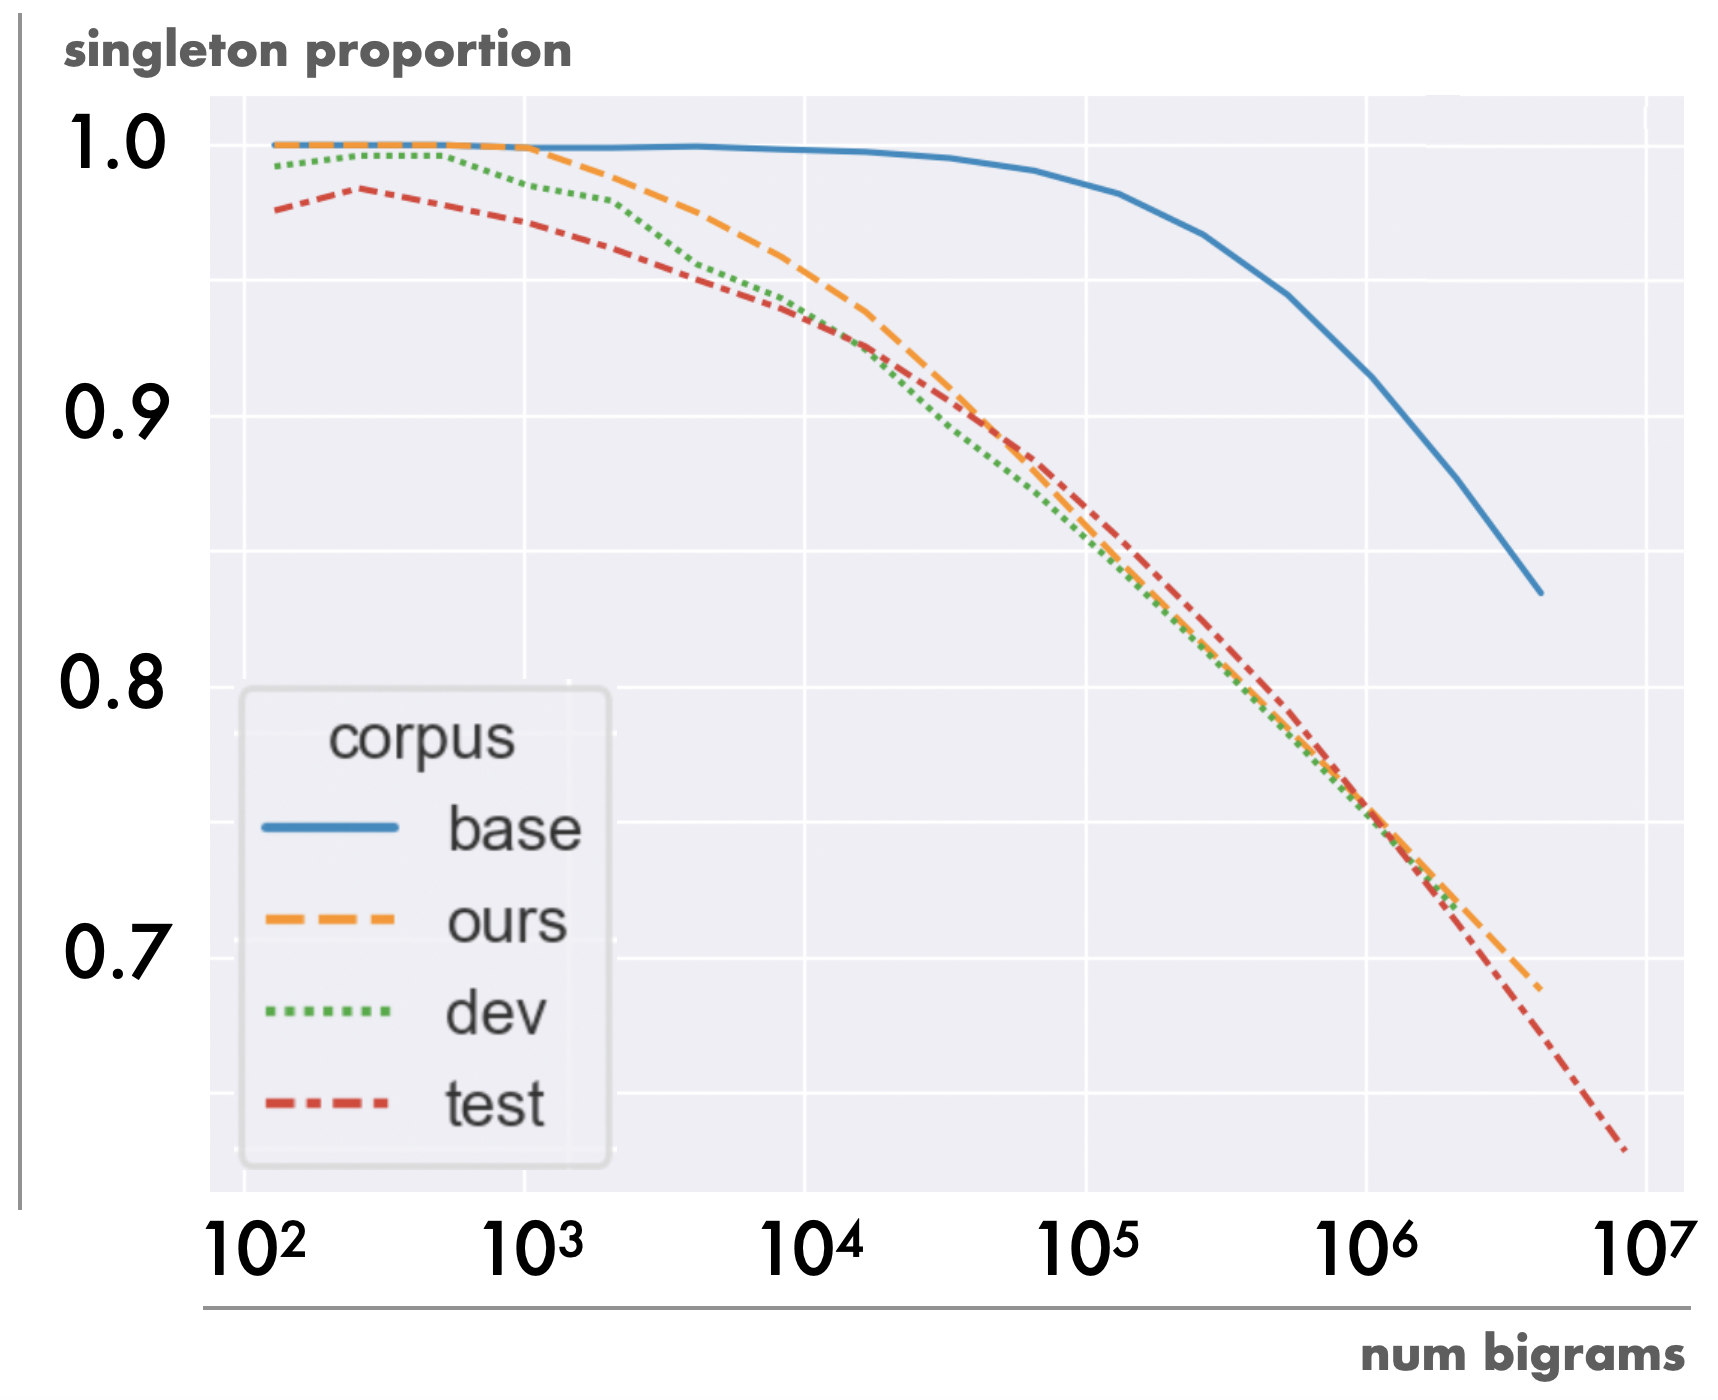
\includegraphics[width=.48\textwidth]{images/sp_curve_test.png}
\caption{Singleton proportion of verb-object dependency bigrams as corpus size increases.}
\label{fig:sp_curve_test}
\end{figure}

\begin{figure}[t]
\centering
\begin{tabular}{ll||ll|ll} 
&&\multicolumn{2}{l|}{singleton}&\multicolumn{2}{l}{type-token}\\
&&\multicolumn{2}{l|}{proportion}&\multicolumn{2}{l}{ratio}\\
\cline{3-6}
&&\texttt{dev}&\texttt{test}&\texttt{dev}&\texttt{test}\\
\hline \hline
amod & base & 0.099 & 0.094 & 0.23 & 0.23 \\
& ours & \textbf{0.0074} & \textbf{0.013} & \textbf{0.016} & \textbf{0.018} \\
\hline
nsubj & base & 0.045 & 0.057 & 0.083 & 0.12 \\
& ours & \textbf{0.0044} & \textbf{0.010} & \textbf{0.014} & \textbf{0.041} \\
\hline
dobj & base & 0.081 & 0.088 & 0.18 & 0.22 \\
& ours & \textbf{0.0081} & \textbf{0.014} & \textbf{0.036} & \textbf{0.054} 
\end{tabular}
\caption{Absolute difference of singleton proportion and type-token ratio between artificial corpora (ours and base) and natural corpora (dev and test), averaged over power-of-two corpora sizes from $2^7$ to $2^{22}$. \label{fig:abs_avg_table}}
\end{figure}

%\begin{figure*}[t]
%\centering
%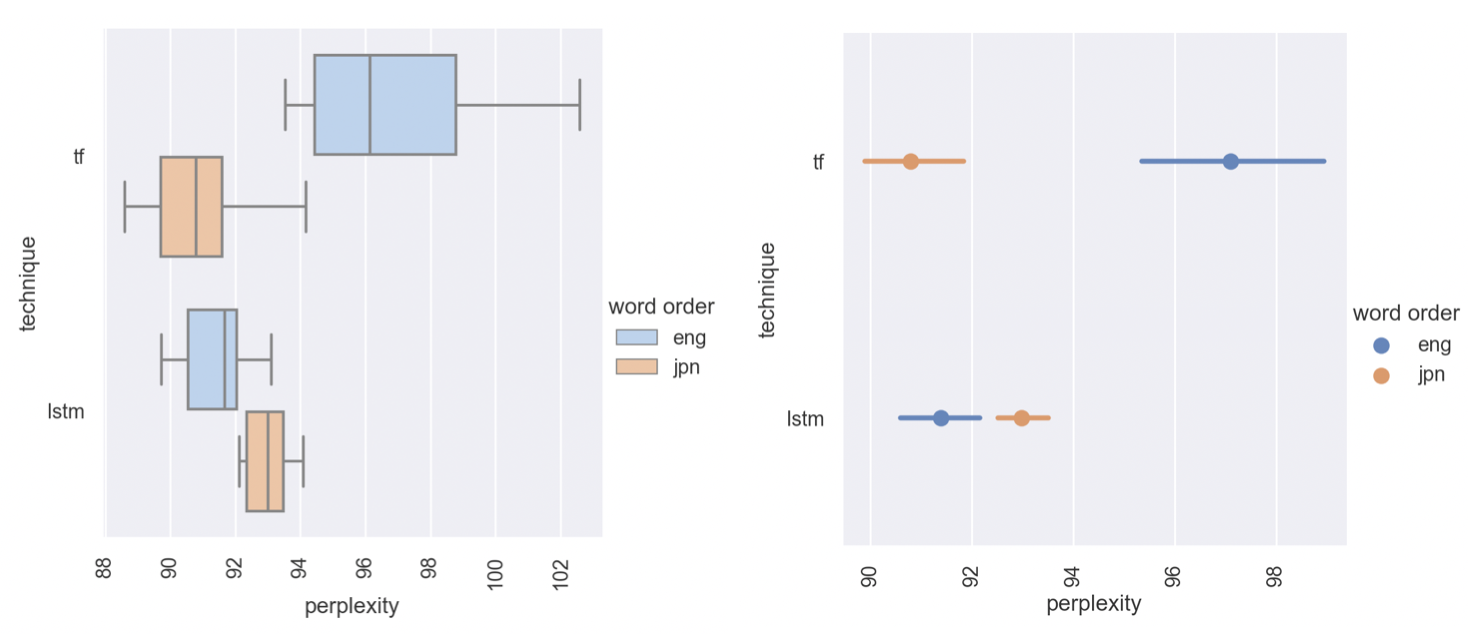
\includegraphics[width=.96\textwidth]{images/results.png}
%\caption{Visualization of experimental results using a box plot (left) and point plot (right). The transformer produces lower-perplexity language models for the artificial languages that follow a Japanese word order, while the LSTM produces lower-perplexity language models for the artificial languages that follow an English word order.}
%\label{fig:results}
%\end{figure*}

\begin{figure}[t]
\centering
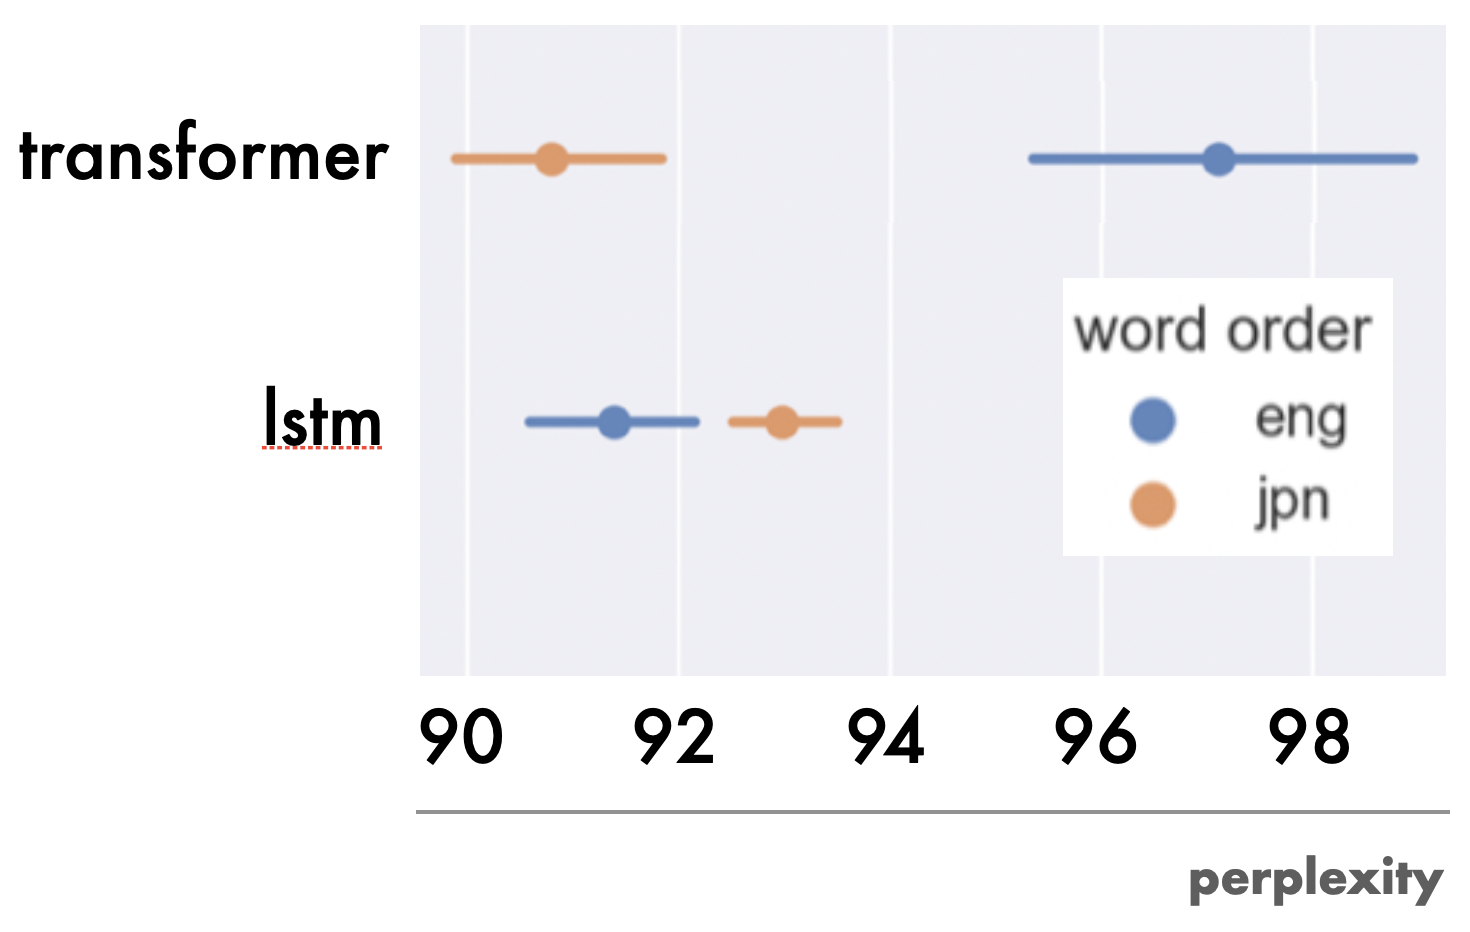
\includegraphics[width=.48\textwidth]{images/boxplot.png}
\caption{Visualization of experimental results using a point plot. The transformer produces lower-perplexity language models for the artificial languages that follow a Japanese word order, while the LSTM produces lower-perplexity language models for the artificial languages that follow an English word order.}
\label{fig:results}
\end{figure}


As a pilot study of our framework, we re-created an experiment performed by \citet{white-cotterell-2021-examining}, who used WCFGs to investigate the inductive biases of neural language models for various word orders exhibited by natural language. We created a WRIG based on their WCFG description, which produces simple declarative sentences with relative clauses, prepositional phrases, and clausal complements. We used a voicebox that assigned concatenations of random syllables to each generic noun, verb, and adjective. It used English prepositions, determiners, and morphology (e.g. verbs with a singular subject were suffixed with the letter ``s''). We set the parameters of our Pitman-Yor processes by specifying discount and strength parameters so that our produced sentences closely matched the type-token ratio and singleton proportion curves of the English side of the WMT 2014 German-English parallel corpus \cite{bojar-etal-2014-findings,luong-etal-2015-effective} for the following dependency bigrams: adjective-noun (amod), verb-subject (nsubj), verb-object (dobj). Figure~\ref{fig:sp_curve_test} compares the singleton proportion curves of verb-object dependencies for our generated corpus, versus the development corpus (WMT 2014 Ger-Eng) and a held-out test corpus: the English side of the JParaCrawl 3.0 Jpn-Eng corpus \cite{morishita2022jparacrawl}. We also compare our corpus statistics to a baseline that attempts to replicate \cite{white-cotterell-2021-examining}, using independent adjective, noun, and verb distributions rather than tied hierarchical Pitman-Yor distributions. Visual inspection shows that the independent baseline is an outlier, unrepresentative of the statistics manifested by natural corpora. We can distill these curves into a single numeric indicator by averaging the absolute difference between an artificial corpus curve (\texttt{ours} or \texttt{base}) and a natural corpus curve (\texttt{dev} or \texttt{test}) for each power of two on the x-axis. Figure~\ref{fig:abs_avg_table} presents these numbers for singleton proportion and the type-token ratio: the statistics for our generated corpus are an order-of-magnitude closer to natural corpora than the baseline.



We created two variants of the WRIG, corresponding to the standard word orders of English and Japanese. For instance, as a head-final language, the Japanese WRIG included the rule\footnote{A brief guide to the referenced indexed nonterminals of the WRIG: $\bnfpn{VP[y_1.y_2]}$ produces a verb phrase with subject count $\bnfpn{y_2}$, whose head is the $\bnfpn{y_1}^{\mathsf{th}}$ verb of the vocabulary. 	$\bnfpn{NP[y_1,y_2]}$ produces a noun phrase with count $\bnfpn{y_2}$, whose head is the $\bnfpn{y_1}^{\mathsf{th}}$ noun of the vocabulary. $\bnfpn{VB[y_1,y_2]}$ produces the $\bnfpn{y_1}^{\mathsf{th}}$ verb of the vocabulary, conjugated for subject count $\bnfpn{y_2}$.}:
\begin{equation*}
\bnfpn{VP[y_1, y_2]} \bnfpo \bnfpn{NP[z_1, z_2]} \bnfsp \bnfpn{VB[y_1, y_2]}
\end{equation*}
and as a head-initial language, the English WRIG included the rule:
\begin{equation*}
\bnfpn{VP[y_1, y_2]} \bnfpo \bnfpn{VB[y_1, y_2]} \bnfsp \bnfpn{NP[z_1, z_2]}
\end{equation*}
Following \cite{white-cotterell-2021-examining}, the WRIGs also differed in:
\begin{itemize}
\item the position of the complementizer in complements, relative to the sentential component
	\item the position of the adposition in adpositional phrases, relative to the adpositional object
	\item the position of a relative clause, relative to the noun it modifies
\end{itemize}

\noindent We generated 1,000,000 sentences for each WRIG variant, and divided these into ten evenly sized corpora. Each corpus of 100,000 sentences was further divided into an 80k-10k-10k train-dev-test partition. On each train set, we trained\footnote{Like \citet{white-cotterell-2021-examining}, we used the \texttt{fairseq} implementation \cite{ott-etal-2019-fairseq} of these language models.} a transformer-based and an LSTM-based language model, resulting in 10 trained language models (LMs) per choice of neural architecture and WRIG. Finally, we evaluated these LMs on the respective test sets. 

For each architecture (transformer and LSTM) and word order (English and Japanese), Figure~\ref{fig:results} visualizes the test perplexity over the ten trials using a point plot\footnote{We used \texttt{seaborn} to generate the plot. A point plot shows the mean of the ten trials (the dot) and the 95\% confidence interval (the line).}. For transformer LMs, we obtained lower perplexity on the languages that followed a Japanese word order. For LSTM LMs, we observed the opposite: a (statistically significant) lower perplexity on the languages that followed an English word order. While these results generally support the findings of \citet{white-cotterell-2021-examining}, \citet{white-cotterell-2021-examining} did not find significant differences between the LSTM LMs. We find it encouraging that our results do not differ wildly from \citet{white-cotterell-2021-examining} (it would be troubling for the prospects of artificial languages if each iterative improvement dramatically reversed the conclusions of the previous iteration). At the same time, we also find it encouraging that the differences between their results and ours offer a possible reconciliation between \citet{white-cotterell-2021-examining} and \citet{ravfogel-etal-2019-studying}, who reported, based on experiments with naturally-derived corpora, that LSTM LMs performed better on SVO (versus SOV) languages.




\section{Conclusion}

With this work, our goal is to enable researchers to more easily develop models for typologically diverse languages, and to investigate under what conditions such models perform effectively. By demonstrating that RIGs (weighted by hierarchical Pitman-Yor processes) can model realistic syntactic and semantic dependencies, we hope to provide some confidence that the framework can prove a useful proxy for real-world data, when such data is not readily available. To facilitate adoption of our framework, we are also releasing an open-source Python package called \texttt{testperanto} for building WRIGs, providing fellow researchers with a means to generate artificial languages that emulate the typology of the natural languages they seek to study. 


%\appendix

%\section{Additional Experimental Details}

%The experiments were run on a single workstation with the following specifications:
%\begin{itemize}
%	\item \textbf{Operating System:} Ubuntu 18.04 	
%	\item \textbf{Processor:} Intel Xeon E5-1650 v4 (6 core)
%	\item \textbf{GPUs:} 4x NVIDIA GeForce GTX 1080Ti
%	\item \textbf{Memory:} 128 GB DDR4 RAM
%\end{itemize}

%\noindent The language models were trained with the following command:

%\noindent
%\small
%\texttt{fairseq-train \\
%  --task language\_modeling \\
%  --arch \{transformer\_lm, lstm\_lm\} \
%  --share-decoder-input-output-embed \
%  --dropout 0.1 \
%  --optimizer adam \
%  --adam-betas '(0.9, 0.98)' \
%  --weight-decay 0.01 \\
%  --clip-norm 0.0 \
%  --lr 0.0005 \
%  --lr-scheduler inverse\_sqrt \
%  --warmup-updates 4000 \
%  --warmup-init-lr 1e-07 \
%  --tokens-per-sample 512 \
%  --sample-break-mode none \\
%  --max-tokens 2048 \
%  --update-freq 16 \
%  --patience 15 \
%  --fp16 \\
%  --max-update 50000}


\bibliography{anthology,custom}
\bibliographystyle{acl_natbib}

\appendix


\end{document}


